\chapter{Experimental analysis}
\label{chapter:exp}


\section{Simulating a crowd sensing campaign}
\label{sec:exp-crowd}

\subsection{Use cases}

In order to simulate a crowd sensing campaign, we require a set of characteristics for the campaign. A campaign can be characterized by the area of interest, the zone from which the data needs to be gathered, the range at which a sensor can measure data and the time the campaign is expected to take place.

A WiFi sensor can detect hotspots at ranges of about 100m, according to the WiFi 802.11 standards\footnote{\url{http://standards.ieee.org/about/get/802/802.11.html}}. In contrast, an air quality sensor can take measurements of the air that directly touches it. For the later one we assume the measurements are relevant for a distance of 3m.

The area of interest can have highly irregular shapes. Consider a park, not only is the outer perimeter of the park often irregular, but a park may contain features that are not accessible to pedestrians such as small lakes. In order to have an accurate representation we extract the zone of interest from Open~Street~Maps\footnote{\url{https://www.openstreetmap.org}}. The simulator takes the given area and the number of participants and generates their movement. We use random walk in order to simulate the movement of the individuals over a period of time.

In order to verify the correctness of our simulator we built a small visualization tool. A NodeJS server offers the simulation data to a JavaScript tool that makes use of the Google~Maps\footnote{\url{https://www.google.ro/maps}} library in order to display the locations of individuals inside the area of interest. An example of the visualization can be observed in Figures \ref{fig:1}. The area of park Herastrau, as described in Open Street Maps, is represented with red and the small white discs represent pedestrians.

\begin{figure}
	\centering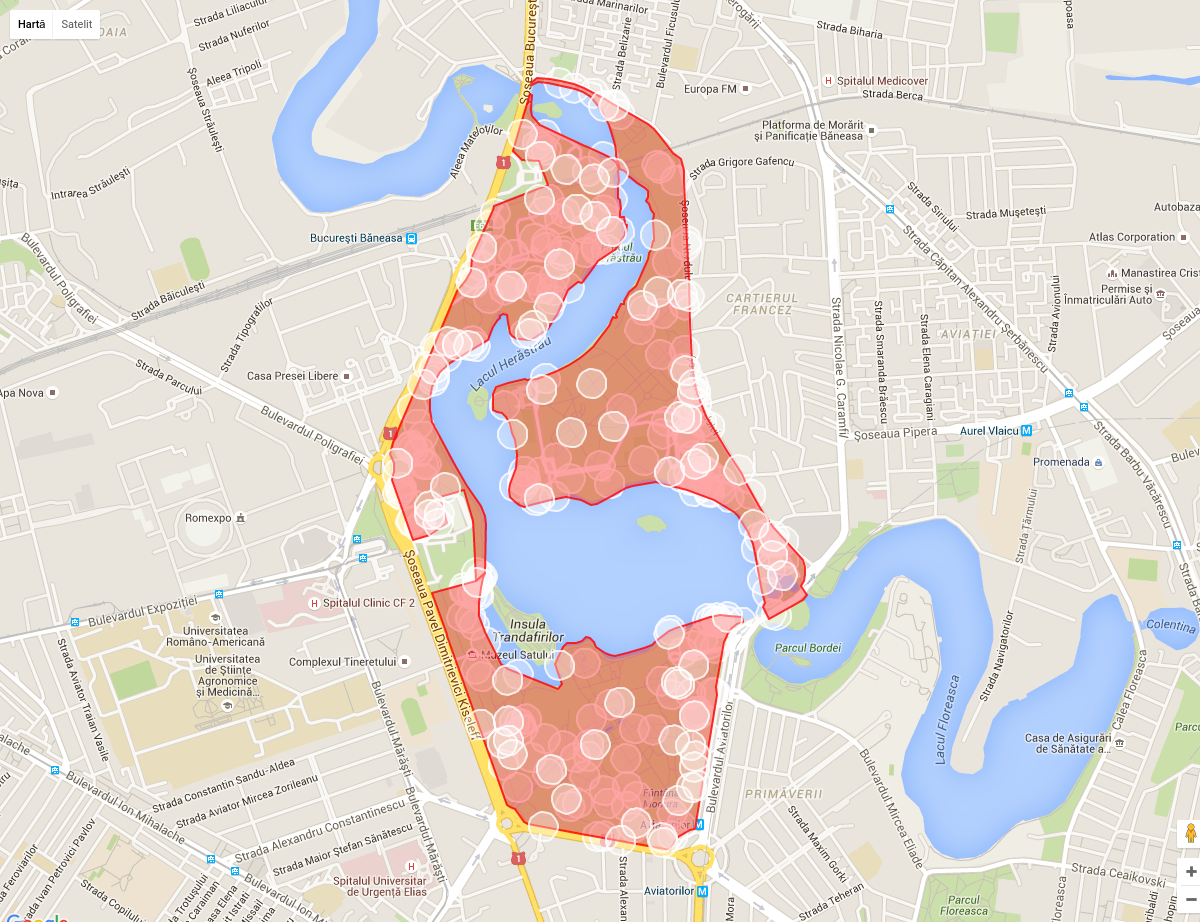
\includegraphics[width=7.5cm]{src/img/Herastrau-100pers-50m.png}
	\caption{Simulation, 100 persons, sensing area radius of 50m}
	\label{fig:1}
\end{figure}

Because the shape of the interest space can be bounded by an irregular polygon, in order to calculate its area, we use grid sampling. We take an outer rectangle that encapsulates the entire area and split it in a grid of 1000 by 1000 cells. We then count the total number of cells that are inside the polygon. Finally, we multiply the total number of cells inside the area of interest with the area of a cell.

To determine if a cell is inside the polygon describing the interest space we use a ray casting algorithm~\cite{roth1982ray}. In ray casting a set of parallel lines are drawn over the rectangle. We start in the upper left corner and use vertical lines. The intersections between these lines and the polygon are calculated. For each cell, if the number of intersections is even, it means the cell is inside the polygon and thus inside the area of interest, otherwise it means the cell is outside.

In order to simulate pedestrians, we randomly choose their starting location as points inside the area of the park. We generate random locations inside the outer rectangle and keep only those that are inside the polygon. In order to determine if the location is inside the space of interest we used the same ray casting method.

To have a more realistic simulation we added movement. Crowdsensing campaigns use pedestrians or even vehicles. In our experiments we focused on spaces such as parks through which only pedestrians can move. We set the same speed of 5km/h for all simulated individuals. The speed was chosen according to~\cite{carey2005establishing}. The movement was simulated using the Random Walk~\cite{pearson1905problem} algorithm. In random walk, pedestrians move in a randomly chosen direction until they reach the edge of the interest space. In our case we consider collisions with any element of the polygons. Because we focus on parks, there can be multiple polygons. As we stated earlier, parks can have features that are not accessible by pedestrians, such as small lakes. Each of these are bounded by a polygon. When we detect a collision for a pedestrian another direction is chosen randomly and the pedestrian continues its movement in the new direction with the same speed.

In order to simulate the data gathering process we use discs of a set radius centered on each of the pedestrians. In reality the shape of the detection area for a sensor is highly irregular. Take WiFi, where the shape of the area in which frames can be correctly received varies with irregularities of the antenna, features of the environment and even weather. Because the shape varies from sensor to sensor and there is no model that describes the irregularities found in nature a disc can be used as an acceptable approximation.

In order to calculate the area of the surface of the interest space covered by at least one of the sensors carried by the pedestrians we use the same grid sampling method. In this case, a cell represents an area that we consider to be covered by a sensor if there exist at least one sensor whose disc covers at least half of the cell. In order to determine if a cell is inside a disc we calculated the Euclidean distance~\cite{deza2009encyclopedia} from the center of the cell to the position of any pedestrian. If, for any pedestrian, this distance is smaller than the sensing radius we consider the cell to be covered by the sensors. This is described in equation \ref{eq:cellcovered}, where $x_c$ and $y_c$ represent the location of the center of the cell and $x_p$ and $y_p$ represent the location of a pedestrian.

\begin{equation}
\forall i; \sqrt{(x_{c}-x_{p_i})^2 + (y_{c}-y_{p_i})^2}<sensingRadius
\label{eq:cellcovered}
\end{equation}

The final goal of the simulation is, given a sensing radius, an area of interest and a time period, to determine the percentage of the area of interest that is covered by sensors. After we count the number of cells covered by the sensors and the number of cells inside the area of interest we use equation \ref{eq:percentagecovered} in order to determine the percentage of the area covered by sensors. For a cell to be considered covered it needs to have been inside the disc of a sensor at any point in time during the simulation.

\begin{equation}
coveredPercentage = \frac{count_{coveredCells}}{count_{spaceOfInterestCells}} *100
\label{eq:percentagecovered}
\end{equation}

\section{Accelerometers}
\label{sec:exp-acc}

\subsection{Use case}

In terms of use cases that can be taken into consideration, which can combine the power of crowd sensing with the low costs and popularity of accelerometers that are embeded in smartphones, there are a multitude of application that can be built. One example can be taking real time readings of the magnited of earth movement caused by earthquakes or other sources of vibration like subways. Another great application can be using accelerometers and crowd sensing to see where users are most likely to enage in phisical activities, so that this area can be further be incrised. Also, smartphones in cars could capture data associated with incidents and using crowd sensing, a map of the most dangerous areas can be made and different actions can be taken to reduce them.

The use case proposed by us, wants to take advantage of the smartphones popularity and integration of inertial sensors to recognize gestures and diferentiate between normal walking and using an elevator or going up or down a stairway. This data gatherd from a large number of smartphones, through crowd sensing will result in a map of stairs and elevators, from which persons with disabilities could use when choosing a path to a destination.

This use case would imply minimal effort in terms of capturing data. The smartphone should be able to identify by itself different context of movement, withouth user input. In terms of security data gathered can be anonimous, as it is important to have a general idea of locations of stairs and elevators, not only for one person.

\subsection{Data acquizition}

For data acquizition an Android application is built, which will help with capturing data from inertial sensors, that will be later used as training and testing datasets. In this phase user input is important, so that datasets are segmented and the segment includes only one event of the following:
 \begin{itemize}
\item stairs up - from the moment one leg leaves the ground, to the moment that the same leg touches the next step in the stairway
\item stairs down - the same of above, only reversed
\item elevator up - will contain only the first part when the elevator is starting to accelerate until it reaches a constant speed
\item elevator down - the same as above, only the elevator is going down
\item non relevant move - to test null rejection, which means that a gesture does not fit any of the above gestures. Can be a step in walkig, running or stanging stil
\end{itemize}

The first step in the data acquisition process will be, it is very important that the phone's orientaion should not give different readings. For this two methods are considered. One is using the acceleration magnitude form the equation \ref{eq:magnitude}, where x, y, z are the acceleration on the coordinates. Although this is a good method for general cases, in the usecase, provided the most movement is happening on the vertical axis, it would mean that the result would only add irelevant noise.

\begin{equation}
a = \sqrt{x^{2} + y^{2} + z^{2}}
\label{eq:magnitude}
\end{equation}

A better solution is proposed by the Android framework and uses the reading from the gravity and magnetic sensors so that a rotation matrix is calculated, which can be used to transform a vector, more specifics the accelerations vector, from the device coordinate system to the world's coordinate system, as you can see in \ref{lst:coord}.

\lstset{language=make,caption=Transforming to world's coordinate system,label=lst:coord}
\begin{lstlisting}
SensorManager.getRotationMatrix(R, I, gravityValues,
magneticValues);
android.opengl.Matrix.invertM(inv, 0, R, 0);
android.opengl.Matrix.multiplyMV(earthAcc, 0, inv, 0,
 linear_acceleration, 0);
// liniar_acceleration matrix will be transofrmed to 
// world's coordinate system
\end{lstlisting}

The second step is to isolate the force of gravity with the low-pass filter and remove the gravity contribution with the high-pass filter.

Another step includes calibration which will be used for normalization of the data. For this reading will be taken in the following cases:
\begin{itemize}
\item phone set on screen, which will be associated with +1g
\item phone set on back, which will be associated with -1g
\item phone droped, for exeample from one hand to another, which will be associated with 0
\end{itemize}

Readings will be normalized so that diferent devices have similar readings using filters like 

https://www.google.ro/webhp?sourceid=chrome-instant&ion=1&espv=2&ie=UTF-8#q=android%20accelerometer%20normalize
http://electronics.stackexchange.com/questions/195796/normalize-values-from-different-mems-3-axis-accelerometers

\subsection{Gesture recognition}

\subsection{Testing}


